% !TeX root = ../tfg.tex
% !TeX encoding = utf8

\chapter{Teoría de Categorías}\label{ch:categorias}

\section{Introducción}

\section{Categorías y functores}

\begin{definicion}\label{def_categoria}
    Una categoría $\mathscr{C}$ consiste en:
    \begin{enumerate}
        \item Una clase $|\mathscr{C}|$ cuyos elementos se llamarán ``objetos de la categoría'';
        \item Para cada par $A,B$ de objetos, un conjunto $\mathscr{C}(A,B)$, conocido como \textit{homset}, cuyos elementos llamaremos ``morfismos'' ó ``flechas'' desde $A$ hasta $B$;
        \item Para cada $A,B,C \in |\mathscr{C}|$, se define una ley de composición:
            \begin{equation}
                \mathscr{C}(A,B) \times \mathscr{C}(B,C) \longrightarrow \mathscr{C}(A,C)
            \end{equation}
        la composición del par $(f,g)$ se notará como $g\circ f$, ó simplemente $gf$;
        \item Para cada objeto $A$, un morfismo $1_{A} \in \mathscr{C}(A,A)$ que llamaremos la identidad en $A$.
    \end{enumerate}
\end{definicion}

En una categoría encontramos los siguientes axiomas o propiedades:

\begin{enumerate}
    \item \textit{Asociatividad: } dados los morfismos $f \in \mathscr{C}(A,B)$, $g \in \mathscr{C}(B,C)$, $h \in \mathscr{C}(C,D)$, la siguiente igualdad se cumple:
        \begin{equation}
            h \circ (g \circ f) = (h \circ g) \circ f.
        \end{equation}
    Esto es, la ley de composición de morfismos es asociativa.    
    \item \textit{Identidad: } dados los morfismos $f \in \mathscr{C}(A,B)$, $g \in \mathscr{C}(B,C)$ la siguiente igualdad se cumple: 
        \begin{equation}
            1_{B} \circ f = f, \quad g \circ 1_{B} = g 
        \end{equation}
\end{enumerate}

\begin{figure}[htpb] % El entorno figure permite añadir el título
    \centering
    \begin{tikzcd}[row sep=2cm, column sep=2cm]
        A \arrow{r}{f} \arrow{d}[left]{h} 
        & B \arrow{d}{g}  \\
        C \arrow{r}{k} 
        & D
    \end{tikzcd}
    \caption{Diagrama conmutativo}
    \label{diag:diagrama-basico}
\end{figure}

Un morfismo $f \in \mathscr{C}(A,B)$ normalmente se representará mediante la notación con flecha $f: A \longrightarrow B$, donde $A$ se conoce como ``dominio'' y $B$ como ``codominio''.
En la situación del diagrama \ref{diag:diagrama-basico}, diremos que dicho diagrama es ``conmutativo'' si se da la igualdad $g \circ f = k \circ h$. El concepto de ``conmutatividad'' se mantiene para diagramas de dimensión aritraria. \\
El morfismo identidad $1_{A}$ de un objeto $A$ es el único morfismo cumpliendo el rol de identidad para la composición de morfismos. Esto es, si $i_{A} \in \mathscr{C}(A,A)$ cumple dicha propiedad, entonces:

\begin{equation}
    1_{A} = 1_{A} \circ i_{A} = 1_{A}
\end{equation}

Una forma importante de construir categorías a partir de una categoría dada se recoge en la siguiente definición.

\begin{definicion} [Categoría opuesta]
    Toda categoría $\mathscr{A}$ tiene una categoría \textit{opuesta} $\mathscr{A}^{op}$ definida:
    \begin{enumerate}
        \item $|\mathscr{A}^{op}| = |\mathscr{A}|$,
        \item $\mathscr{A}^{op}(B,A) = \mathscr{A}(A,B) \, \, \, , \forall A,B \in |\mathscr{A}^{op}|$,
        \item En cuanto a la ley de composición, si tenemos $f \in \mathscr{C}^{op}(A,B)$ y $g \in \mathscr{C}^{op}(B,C)$ esto se traduce en $f \in  \mathscr{C}(B,A)$ y $g \in \mathscr{C}(C,B)$. Como $\mathscr{C}$ es una categoría, podemos aplicar su ley de composición de forma que el morfismo $g \circ f \in \mathscr{C,A}$ está bien definido. Por la forma de construir $\mathscr{C}^{op}$, obtenemos $f \circ g \in \mathscr{C}^{op}(A,C)$, quedando bien definida la ley de composición para dichar categoría.
        \item Dada la forma en que se han definido los \textit{homsets} en $\mathscr{C}^{op}$, es evidente que existe, para todo objeto $A \in \mathscr{C}^{op}$, su identidad.
    \end{enumerate}
\end{definicion}

Una propiedad importante en teoría de categorías es el \textit{principio de dualidad}, que relaciona las propiedades que se dan en una categoría $\mathscr{A}$ y su opuesta $\mathscr{A}^{op}$.

Veamos algunos ejemplos:

\begin{ejemplo}
    \textbf{Set: } 
    \begin{itemize}
        \item \textbf{Objetos: } Conjuntos
        \item \textbf{Morfismos: } funciones entre conjuntos
    \end{itemize}
\end{ejemplo}

\begin{ejemplo}
    \textbf{Top: } 
    \begin{itemize}
        \item \textbf{Objetos: } Espacios topológicos
        \item \textbf{Morfismos: } funciones continuas
    \end{itemize}
\end{ejemplo}

\begin{ejemplo}
    \textbf{Grp: } 
    \begin{itemize}
        \item \textbf{Objetos: } Grupos
        \item \textbf{Morfismos: } homomorfismos de grupos
    \end{itemize}
\end{ejemplo}

\begin{ejemplo}
    Sea $I \in \mathscr{C}$ definimos la categoría de flechas sobre $I$, notada como $\mathscr{C}/I$, como sigue:
    \begin{itemize}
        \item \textbf{Objetos: } las flechas cuyo codominio es $I$. Se notarán como $(A,f)$, donde $A$ es el dominio y $f$ el morfismo que llega a $I.$
        
        \item \textbf{Morfismos: } un morfismo entre dos objetos $(A,f)$ y $(B,g)$ es un morfismo $h: A \longrightarrow B$ en $\mathscr{C}(A,B)$ cumpliendo $h \circ g = f$. Esto es, el diagrama \ref{diag:traingulo_hacia} conmuta. La ley de composición y la identidad para un objeto en $\mathscr{C}/I$ son propiedades triviales a partir de las proporcionadas por $\mathscr{C}$.
    \end{itemize}
\end{ejemplo}

\begin{figure}[htpb]
    \centering
    \begin{tikzcd}[row sep=1cm, column sep=1cm]
        A \arrow{dr}[below left]{f} \arrow{rr}{h} 
        & & B \arrow{ld}{g}  \\
        & I
    \end{tikzcd}
    \caption{Triángulo conmutativo}
    \label{diag:traingulo_hacia}
\end{figure}

\begin{ejemplo}
    Siguiendo la misma idea que en el ejemplo anterior, definimos la categoría de morfismos que parten del objeto $I$ de $\mathscr{C}$, notada como $I / \mathscr{C}$ como sigue: 
    \begin{itemize}
        \item \textbf{Objetos: } las flechas cuyo dominio es $I$. Se notarán como $(f,A)$ donde $f$ es el morfismo que parte de $I$ y $A$ es el codominio.
        
        \item \textbf{Morfismos: } un morfismo entre dos objetos $(f,A)$ y $(g,B)$ es un morfismo $h: A \longrightarrow B$ en $\mathscr(C)(A,B)$ cumpliendo $h \circ f = g$. Esto es, el diagrama \ref{diag:traingulo_desde} conmuta.
    \end{itemize}
\end{ejemplo}

\begin{figure}[htpb]
    \centering
    \begin{tikzcd}[row sep=1cm, column sep=1cm]
        & I \arrow{dl}[above]{f} \arrow{dr}{g} & \\
        A \arrow{rr}[below]{h} & & B
    \end{tikzcd}
    \caption{Triángulo conmutativo}
    \label{diag:traingulo_desde}
\end{figure}

\begin{ejemplo}
    Definimos ahora la categoría de flechas de una categoría $\mathscr{C}$, notada como $\textbf{Ar}(\mathscr{C})$ de la siguiente forma:
    \begin{itemize}
        \item \textbf{Objetos: } todas las flechas de $\mathscr{C}$
        \item \textbf{Morfismos: } un morfismo de un objeto $(f: A \longrightarrow B)$ a $(g: C \longrightarrow D)$ es un par $(h: A \longrightarrow C, k: B \longrightarrow D)$ de morfismos de $\mathscr{C}$ cumpliendo $k \circ f = h \circ g$ (ver diagrama \ref{diag:diagrama-flechas})
    \end{itemize}
\end{ejemplo}

\begin{figure}[htpb] % El entorno figure permite añadir el título
    \centering
    \begin{tikzcd}[row sep=2cm, column sep=2cm]
        A \arrow{r}{f} \arrow{d}[left]{h} 
        & B \arrow{d}{k}  \\
        C \arrow{r}{g} 
        & D
    \end{tikzcd}
    \caption{Morfismo de flechas}
    \label{diag:diagrama-flechas}
\end{figure}

Una vez definido el concepto de categoría y sus principales propiedades, veamos ahora el concepto que recoge las correspondencias entre categorías.

\begin{definicion}
    Un functor $F$ de una categoría $\mathscr{A}$ a una categoría $\mathscr{B}$ consiste en:

    \begin{enumerate}
        \item una función \begin{equation}|\mathscr{A}| \longrightarrow |\mathscr{B}| \end{equation} entre las clases de objetos de las categorías; la imagen de un objeto $A \in \mathscr{A}$ se nota $F(A)$ o simplemente $FA$.

        \item para cada $A, A' \in \mathscr{A}$, una función \begin{equation}\mathscr{A}(A,A') \longrightarrow \mathscr{B}(FA,FA') \end{equation}
        la imagen de un morfismo $f \in \mathscr{A}(A,A')$ se nota como $F(f)$ o simplemente $Ff$.
    \end{enumerate}
    \label{functor}

 Los siguientes axiomas aseguran que los functores respeten la estructura subyacente de las categorías donde se definen.
  \begin{enumerate}
        \item para cada par de morfismos $f \in \mathscr{A}(A,A')$, $g \in          \mathscr{A}(A',A''): $ \begin{equation} F(g \circ f) = F(g) \circ F(f)   \end{equation}

        \item para cada $A \in \mathscr{A}$ \begin{equation}
            F(1_{A}) = 1_{FA}
        \end{equation}
    \end{enumerate} 

\end{definicion}

\begin{observacion}
    Se puede definir una ley de composición para functores de la siguiente forma. Sean functores $F: \mathscr{A} \longrightarrow \mathscr{B}$ y $G: \mathscr{B} \longrightarrow \mathscr{C}$ composables, se define el nuevo functor $G \circ F: \mathscr{A} \longrightarrow \mathscr{C}$:

    \begin{enumerate}
        \item Dado $A \in \mathscr{A}$, su imagen por el functor composición se define como $(G \circ F)(A) = G(F(A))$.
        \item Dado $f \in \mathscr{C}(A,B)$, su imagen por el functor composición se define como $(G \circ F)(f) = G(F(f))$.
        \item Sean $ f \in \mathscr{A}(A, B) $ y $ g \in \mathscr{B}(B, C) $. Entonces,
        $$
            (G \circ F)(g \circ f) = G(F(g \circ f)).
        $$
        Dado que $ F $ es un functor de $ \mathscr{A} $, respeta la composición de morfismos, por lo que
        $$
            G(F(g \circ f)) = G(F(g) \circ F(f)).
        $$
        Además, como $ G $ es un functor de $ \mathscr{B} $, también respeta la composición, lo que implica
        $$
            G(F(g) \circ F(f)) = G(F(g)) \circ G(F(f)).
        $$
        En conclusión,
        $$
            (G \circ F)(g \circ f) = G(F(g)) \circ G(F(f)).
        $$
        
    \end{enumerate}

    De esta forma hemos probado que se puede definir el functor composición de dos functores.

\end{observacion}

\begin{observacion}
    Una vez probada la correcta definición de la composición de functores, encontramos las siguientes propiedades de dicha ley:
    \begin{enumerate}
        \item \textit{Asociatividad: } Dados los functores $F: \mathscr{A} \longrightarrow \mathscr{B}$, $G: \mathscr{B} \longrightarrow \mathscr{C}$ y $H: \mathscr{C} \longrightarrow \mathscr{D}$, se cumple: \begin{equation}
            H \circ (G \circ F) = (H \circ G) \circ F   
        \end{equation}
        \item \textit{Identidad: } Para cada categoría $\mathscr{A}$ existe un functor identidad $id_A: \mathscr{A} \longrightarrow \mathscr{A}$ (cuya definición es evidente) de forma que si $F: \mathscr{A} \longrightarrow \mathscr{B}$ es otro functor, se cumple \begin{equation}
            F \circ id_{\mathscr{A}} = id_{\mathscr{B}} \circ F 
        \end{equation} 
    \end{enumerate}
\end{observacion}

A primera vista, podría parecer que las categorías, consideradas como objetos, y los functores, vistos como morfismos entre ellas, satisfacen todos los axiomas necesarios para formar una categoría. Sin embargo, es importante recordar que, para que una colección de morfismos entre dos objetos constituya una categoría, dichos morfismos deben formar un conjunto. En el caso de las categorías y los functores, esto implicaría que el conjunto de todos los functores entre dos categorías dadas debe ser, a su vez, un conjunto. No obstante, esta condición no siempre se cumple, ya que en muchos casos la colección de functores entre dos categorías puede ser demasiado grande para ser un conjunto. Las razones detrás de esto exceden el alcance de este trabajo.

Veamos algunos ejemplos de functores:

\begin{ejemplo}
    El ``forgetful functor'' (o functor olvidadizo, haciendo una traducción literal) $U: \textbf{Ab} \longrightarrow \textbf{Set} $ de la categoría de grupos abelianos a la categoría de conjuntos, lleva un grupo $(G,+)$ en su conjunto asociado $G$ y un homomorfismo de grupos $f$ en una función entre los conjuntos asociados $f$. Debe su nombre a que dicho functor ``olvida'' la estructura subyacente de grupo.
    \label{ej:forgetful}
\end{ejemplo}

\begin{ejemplo}
     La categoría $\textbf{Top}_{*}$ de espacios topológicos con punto base tiene como objetos duplas $(X,x_{0})$ donde:
    \begin{itemize}
        \item $X$ es un espacio topológico.
        \item $x_{0} \in X$ es un punto base de dicho espacio 
    \end{itemize}
    Los morfismos de $\textbf{Top}_{*}$ son funciones $f: (X,x_{0}) \longrightarrow (Y,y_{0})$ cumpliendo:
    \begin{itemize}
        \item $f$ es una función continua entre $X$ e $Y$.
        \item $f(x_{0}) = y_{0}$ 
    \end{itemize}
    El grupo fundamental se puede definir como un functor $\pi_{1}: \textbf{Top}_{*} \longrightarrow \textbf{Grp} $ que asigna a cada espacio con punto base $(X,x_{0})$ su grupo fundamental $\pi_{1}(X,x_{0})$, y a cada función continua entre espacios base $f: (X,x_{0}) \longrightarrow (Y,y_{0})$ el homomorfismo de grupos asociado $f_{*}: \pi_{1}(X,x_{0}) \longrightarrow \pi_{1}(Y,y_{0})$
\end{ejemplo}

\begin{ejemplo}
    El functor $\mathcal{P}: \textbf{Set} \longrightarrow \textbf{Set}$ lleva un conjunto $X$ en su conjunto potencia $\mathcal{P}(X)$ y una función $f: X \longrightarrow Y$ a una función $\mathcal{P}(f): \mathcal{P}(X) \longrightarrow \mathcal{P}(Y)$ que asigna a cada subconjunto $A \subseteq X$ el subconjunto $f(A) \subseteq Y$, esto es $f(A) = \{f(a) : a \in A\} \subseteq Y$.
    \label{ejemplo:potencia}
\end{ejemplo}

\begin{ejemplo}
    Otro functor fundamental en teoría de categorías es el \textbf{functor representable}. Dada una categoría $\mathscr{C}$ y un objeto $C \in \mathscr{C}$, se define el funtor
    \begin{equation}
        \mathscr{C}(C, -): \mathscr{C} \longrightarrow \mathbf{Set},
    \end{equation}
    que asigna a cada objeto $A \in \mathscr{C}$ el conjunto $\mathscr{C}(C, A)$ de morfismos de $C$ a $A$ en la categoría $\mathscr{C}$. 

    Para cada par de objetos $A, B \in \mathscr{C}$ y un morfismo $f: A \longrightarrow B$, se define la acción del functor sobre $f$ como una función entre los conjuntos $\mathscr{C}(C, A)$ y $\mathscr{C}(C, B)$. Específicamente, si denotamos esta función como $\phi: \mathscr{C}(C, A) \longrightarrow \mathscr{C}(C, B)$, entonces, para cada $g \in \mathscr{C}(C, A)$, se define
    $$
    \mathscr{C}(C,-)(f) = \phi(g) = f \circ g \in \mathscr{C}(C, B).
    $$

    Este functor se denomina \textbf{representable} porque está completamente determinado por el objeto $C$. En otras palabras, el objeto $C$ ``representa'' al functor en el sentido de que, al conocer $C$ y cómo se relaciona con los demás objetos y morfismos de $\mathscr{C}$, podemos reconstruir completamente el functor $\mathscr{C}(C, -)$. 
    \label{ej:func_repre}
\end{ejemplo}

Definimos ahora un concepto central en este trabajo.

\begin{definicion} [Functor contravariante]
    Un functor contravariante $F$ de una categoría $\mathscr{A}$ a una categoría $\mathscr{B}$ consiste en:

    \begin{enumerate}
        \item una función \begin{equation}|\mathscr{A}| \longrightarrow |\mathscr{B}| \end{equation} entre las clases de objetos de las categorías; la imagen de un objeto $A \in \mathscr{A}$ se nota $F(A)$ o simplemente $FA$.

        \item para cada $A, A' \in \mathscr{A}$, una función \begin{equation}\mathscr{A}(A,A') \longrightarrow \mathscr{B}(FA',FA) \end{equation}
        la imagen de un morfismo $f \in \mathscr{A}(A,A')$ se nota como $F(f)$ o simplemente $Ff$.
    \end{enumerate}

Las siguientes propiedades aseguran que los functores respeten la estructura subyacente de las categorías donde se definene.
  \begin{enumerate}
        \item para cada par de morfismos $f \in \mathscr{A}(A,A')$, $g \in          \mathscr{A}(A',A''): $ \begin{equation} F(g \circ f) = F(f) \circ F(g)   \end{equation}

        \item para cada $A \in \mathscr{A}$ \begin{equation}
            F(1_{A}) = 1_{FA}
        \end{equation}
    \end{enumerate}  
\end{definicion}

Para evitar confusiones, enfatizaremos que estamos trabajando con un functor como el definido en \ref{functor} llamándolo functor \emph{covariante}. Un functor contravariante $F: \mathscr{A} \longrightarrow \mathscr{B}$ es un functor covariante entre las categorías $\mathscr{A}^{op}$ y $\mathscr{B}$.

\subsubsection{Ejemplos}

Veamos algunos ejemplos de functores contravariantes.

\begin{ejemplo}
    Análogo al functor representable definido en \ref{ej:func_repre}, encontramos el siguiente functor contravariante:

    Dada una categoría $\mathscr{C}$ y un objeto $C \in \mathscr{C}$, se define el functor \begin{equation}
        \mathscr{C}(-,C): \mathscr{C} \longrightarrow Set
    \end{equation} que asocia a cada objeto $A \in \mathscr{C}$, el objeto $\mathscr{C}(A,C)$ de la clase \textbf{Set}. \\
    Si $f: A \longrightarrow B$ es un morfismo en $\mathscr{C}$, la acción  del functor contravariante sobre $f$ será una función entre conjuntos de la siguiente forma: 
    \begin{equation}
        \mathscr{C}(-,C)(f) = \psi: \mathscr{C}(B,C) \longrightarrow \mathscr{C}(A,C)
    \end{equation} de forma que para cada $g \in \mathscr{C}(B,C)$ obtenemos un morfismo $g \circ f: A \longrightarrow C$, esto es, $g \circ f \in \mathscr{C}(A,C).$    
\end{ejemplo}

\section{Transformaciones naturales}
En matemáticas, es común comenzar estudiando los objetos y, posteriormente, analizar las transformaciones entre ellos. En el apartado anterior, hemos visto cómo los functores ``transforman'' una categoría en otra, preservando su estructura categórica. Ahora, nos proponemos dar un paso más: considerar a los functores como objetos y definir transformaciones entre ellos que respeten las estructuras categóricas subyacentes.

\begin{figure}[htpb]
    \centering
    \begin{tikzcd}[row sep=2cm, column sep=2cm]
        FA \arrow{r}{\alpha_{A}} \arrow{d}[left]{F(f)} 
        & GA \arrow{d}{G(f)}  \\
        FA' \arrow{r}{\alpha_{A'}} 
        & GA'
    \end{tikzcd}
    \caption{Diagrama conmutativo}
    \label{diag:trans_natural}
\end{figure}

\begin{definicion}
    Sean dos functores $F,G: \mathscr{A} \longrightarrow \mathscr{B}$ de una categoría $\mathscr{A}$ a una categoría $\mathscr{B}$. Una transformación natural $\alpha: F \Rightarrow G$ de $F$ a $G$ es una clase de morfismos $(\alpha_A:FA \longrightarrow GA)_{A\in \mathscr{A}}$ de $\mathscr{B}$ indexada por los elementos de $\mathscr{A}$ cumpliendo que para cada morfismo $f: A \longrightarrow A'$ se cumple \begin{equation}
        G(f) \circ \alpha_{A} = \alpha_{A'} \circ F(f)
    \end{equation}
    (ver diagrama \ref{diag:trans_natural})
    \label{t_natural_1}
\end{definicion}

%\begin{figure}[htpb]
%    \centering
%    \begin{tikzcd}[row sep=huge]
%        \mathscr{A}
%        \arrow[bend left=65]{r}{F}
%        \arrow[r, "G", name=G]
%        \arrow[r, bend right=65, "H", name=H, swap]
%        \arrow[from=F.south-|G,to=G,Rightarrow,shorten=2pt,"\alpha"] 
%        \arrow[from=G,to=H.north-|G,Rightarrow,shorten=2pt,"\beta"] &
%        \mathscr{B}.
%    \end{tikzcd}
%\end{figure}


\begin{definicion}
        Dados $F,G,H$ functores de $\mathscr{A}$ a $\mathscr{B}$ y $\alpha: F \Rightarrow G$, $\beta: G \Rightarrow H$ se define la composición (vertical) de transformaciones naturales, $(\beta \circledcirc \alpha)_{A}: F \Rightarrow H$, mediante la fórmula \begin{equation}
        (\beta \circledcirc \alpha)_{A} = \beta_{A} \circ \alpha_{A}
    \end{equation}
    
    Esta composición cumple:
    
    \begin{enumerate}
        \item \textit{Asociatividad: } Dados $F,G,H, K$ functores de $\mathscr{A}$ a $\mathscr{B}$ y $\alpha: F \Rightarrow G$, $\beta: G \Rightarrow H$, $\delta: H \Rightarrow K$ transformaciones naturales, se cumple: \begin{equation}
            \delta \circ (\beta \circ \alpha) = (\delta \circ \beta) \circ \alpha
        \end{equation} 
        \item \textit{Identidad: }  Para cada functor $F: \mathscr{A} \longrightarrow \mathscr{B}$ existe una transformación natural $id_{F}: F \Rightarrow F$ que cumple el papel de identidad para la composición, de forma que si $G: \mathscr{A} \longrightarrow \mathscr{B}$ es otro functor y $\alpha: F \Rightarrow G$ es una transformación natural: \begin{equation}
            \alpha \circ id_{F} = id_{G} \circ \alpha
        \end{equation}
    \end{enumerate}
\end{definicion}

De manera análoga a lo discutido previamente en el contexto de las categorías y los functores, observamos que los functores entre las categorías $\mathscr{A}$ y $\mathscr{B}$ pueden ser considerados como objetos, mientras que las transformaciones naturales se interpretan como morfismos entre dichos objetos. Ambas estructuras satisfacen los axiomas que definen una categoría. Sin embargo, al igual que en el caso de los functores, no podemos asegurar que el conjunto de todas las transformaciones naturales entre dos functores sea efectivamente un conjunto. Bajo ciertas condiciones adicionales, esta propiedad se cumple, y los functores junto con sus transformaciones naturales forman una categoría.

Una forma intuitiva de entender las transformaciones naturales es la siguiente: al aplicar un functor a una categoría, asociamos a cada objeto un objeto y a cada morfismo un morfismo. En contraste, en una transformación natural, a cada objeto $A \in \mathscr{A}$ le asignamos un morfismo $\alpha_A$, y a cada morfismo $f: A \longrightarrow A'$ le asignamos un diagrama conmutativo, como el mostrado en el diagrama \ref{diag:trans_natural}. Por lo tanto, si consideramos las categorías como objetos de dimensión $0$, los functores como objetos de dimensión $1$, entonces las transformaciones naturales pueden interpretarse como objetos de dimensión $2$.

Veamos algunos ejemplos de transformaciones naturales.

\begin{ejemplo}
    Sean el functor potencia en la categoría \textbf{Set}, definido en \ref{ejemplo:potencia}, y el functor identidad $id: \textbf{Set} \longrightarrow \textbf{Set}$. La transformación natural $\alpha: id \Rightarrow \mathcal{P}$ definida como $\alpha_{E}: E \longrightarrow \mathcal{P}(E)$ lleva cada elemento $x \in E$ al \textit{singleton} ${x} \in \mathcal{P}(E)$.
\end{ejemplo}

\begin{ejemplo}
    Sea una categoría $\mathscr{C}$ y un morfismo $f:A \longrightarrow B$ de $\mathscr{C}$. De los siguientes functores representables obtenemos una transformación natural $\mathscr{C}(f,-) : \mathscr{C}(B,-) \Rightarrow \mathscr{C}(A,-)$  que asocia a cada objeto $C \in \mathscr{C}$ una función entre conjuntos $\mathscr{C}(f,-)_{C}: \mathscr{C}(B,C) \longrightarrow \mathscr{C}(A,C)$ definida como \begin{equation}
        \mathscr{C}(f,-)_{C}(g) = g \circ f
    \end{equation}
\end{ejemplo}

La definición hecha en \ref{t_natural} corresponde a transformaciones naturales de functores covariantes. De forma análoga se definen las transformaciones naturales entre functores contravariantes. 

\begin{figure}[htpb]
    \centering
    \begin{tikzcd}[row sep=2cm, column sep=2cm]
        FA \arrow{r}{\alpha_{A}} 
        &  GA \\
        FA' \arrow{r}{\alpha_{A'}} \arrow{u}[left]{F(f)}
        & GA' \arrow{u}{G(f)} 
    \end{tikzcd}
    \caption{Diagrama conmutativo}
    \label{diag:trans_natural_contra}
\end{figure}

\begin{definicion}
    Sean dos functores contravariantes $F,G: \mathscr{A} \longrightarrow \mathscr{B}$ de una categoría $\mathscr{A}$ a una categoría $\mathscr{B}$. Una transformación natural $\alpha: F \Rightarrow G$ de $F$ a $G$ es una clase de morfismos $(\alpha_A:FA \longrightarrow GA)_{A\in \mathscr{A}}$ cumpliendo que para cada morfismo $f: A \longrightarrow A'$ se cumple \begin{equation}
        G(f) \circ \alpha_{A'} = \alpha_{A} \circ F(f)
    \end{equation}
    (ver diagrama \ref{diag:trans_natural_contra})
    \label{t_natural}    
\end{definicion}

\section{Subcategorías}

\begin{definicion}
    Sea el functor $F: \mathscr{A} \longrightarrow \mathscr{B}$ y para cada par de objetos $A,A' \in \mathscr{A}$ la función \begin{equation}
        \mathscr{A}(A,A') \longrightarrow \mathscr{B}(FA,FA'), \, \, \, f \mapsto Ff
    \end{equation}
    \begin{enumerate}
        \item Decimos que el functor F es \textit{faithful} si la función definida arriba es inyectiva para cada $A,A'$.
        \item Decimos que el functor F es \textit{full} si la función definida arriba es sobreyectiva para cada $A,A'$.
        \item Decimos que el functor F es \textit{full} y \textit{faithful} si la función definida arriba es biyectiva para cada $A,A'$.
        \item El functor F es un isomorfismo de categorías cuando es \textit{full} y \textit{faithful} e induce una biyección $|\mathscr{A}| \longrightarrow |\mathscr{B}|$ entre las clases de objetos.
    \end{enumerate}
\end{definicion}

Damos ahora el concepto de subcategoría:

\begin{definicion}
    Una subcategoría $\mathscr{B}$ de una categoría $\mathscr{A}$ consiste en:
    \begin{enumerate}
        \item Una subclase $|\mathscr{B}| \subseteq |\mathscr{A}|$ de la clase de objetos,
        \item Para cada par de objetos $A,A' \in \mathscr{B}$, un subconjunto $\mathscr{B}(A,A') \subseteq \mathscr{A}(A,A')$ de forma que 
        \begin{enumerate}
            \item $f \in \mathscr{B}(A,A')$ y $g \in \mathscr{B}(A',A'') \implies g \circ f \in \mathscr{B}(A,A''),$ 
            \item $\forall A \in \mathscr{B}, 1_{A} \in \mathscr{B}(A,A).$
        \end{enumerate}

    \end{enumerate}
    De forma evidente, una subcategoría es una categoría. Además, una subcategoría $\mathscr{B}$ de $\mathscr{A}$ induce un functor inclusion $\mathscr{B} \longrightarrow \mathscr{A}$ que es \textit{faithful}.
\end{definicion}

Veamos un ejemplo interesante:
\begin{ejemplo}
    Recordemos el \textit{forgetful functor} definido en \ref{ej:forgetful} que asignaba a cada grupo $G \in \textbf{Grp}$ su estructura subyacente de conjunto en la categoría $\textbf{Set}$. Es evidente que se cumple $|Grp| \subseteq |Set|$. Además, para cada dos grupos $G, H \in \textbf{Grp}$, el conjunto de homomorfismos de grupos entre ellos, $\textbf{Grp}(G,H)$ está contenido en el conjunto $\textbf{Set}(G,H)$ de funciones entre los conjuntos subyacentes. Por tanto \textbf{Grp} es una subcategoría de $\textbf{Set}$, y el \textit{forgetful functor} define la inclusión entre ambas categorías (esto es, el \textit{forgetful functor} es \textit{faithful}).
\end{ejemplo}

\section{Límites y colímites}

Vamos a empezar viendo algunos ejemplos comunes del concepto de límite, con el objetivo de tener una visión más general una vez enunciemos la definición.


\begin{definicion} [Producto] \label{definicion_producto} 
    Sea $\mathscr{C}$ una categoría y $A,B \in \mathscr{C}$ dos objetos. Un producto de $A,B$ consiste en un objeto $P$ y morfismos:

    \begin{center}
        \begin{tikzcd}[row sep=1cm, column sep=1cm]
            &  P \arrow{ld}[swap]{p_{A}} \arrow{rd}{p_{B}} & \\
            A & & B
        \end{tikzcd}
    \end{center}
    de forma que para cada objeto $Q$ y morfismos


    \begin{figure}[htpb]
        \centering
        \begin{tikzcd}[row sep=1cm, column sep=1cm]
            &  Q \arrow{ld}[swap]{q_{A}} \arrow{rd}{q_{B}} & \\
            A & & B
        \end{tikzcd}
        \label{diag:producto}
    \end{figure}
        
    en $\mathscr{C}$, existe un \textbf{único} morfismo $r: Q \longrightarrow P$ tal que el diagrama \ref{diag:universal-producto} conmuta.

    \begin{figure}[htpb]
        \centering
        \begin{tikzcd}[row sep=1cm, column sep=1cm]
            & Q \arrow[dashed]{d}[description]{\exists! \ r} \arrow{ld}[swap]{q_A} \arrow{rd}{q_B} & \\
            A & P \arrow{l}[swap]{p_{A}} \arrow{r}{p_{B}} & B
        \end{tikzcd}
        \caption{Propiedad universal del producto}
        \label{diag:universal-producto}
    \end{figure} 
    
    Esto se conoce como propiedad universal del producto. El producto es el objeto (y morfismos) ``más general'' que cumple las condiciones de las proyecciones $p_{A}$ y $p_{B}$.
    Lo notaremos como $(P, p_{A}, p_{B})$   
\end{definicion}

\begin{proposicion} \label{producto-salvo-iso}
    En una categoría $\mathscr{C}$ el producto de dos objetos $A,B \in \mathscr{C}$ (si existe) es único salvo isomorfismo.
\end{proposicion}
\begin{proof}
    Notar que el producto no siempre existe.  Por ejemplo, consideremos la categoría discreta 
    $\mathscr{A}$ formada únicamente por los objetos $A$ y $B$. En esta categoría no puede existir el producto de $A$ y $B$. 

    Veamos ahora la unicidad salvo isomorfismo. Consideremos en la categoría $\mathscr{C}$ dos productos $(P, p_A, p_B)$ y $(Q, q_A, q_B)$ de los
    objetos $A,B \in \mathscr{C}$. Como $(P, p_A, p_B)$ es un prodcuto, existe un único morfismo $r: Q \longrightarrow P $ cumpliendo que 
    $q_A = p_A \circ r$ y  $q_B = p_B \circ r$. De forma análoga, como $(Q, q_A, q_B)$ es un producto, existe un único morfismo 
    $s: P \longrightarrow Q $ cumpliendo $p_A = q_A \circ s$ y  $p_B = q_B \circ s$.

    Tomando ahora $(P, p_{A}, p_{B})$ como producto y como una tripleta cualquiera, por la propiedad universal del producto, existe un único morfismo
    $t: P \longrightarrow P $ de forma que $p_A \circ t = p_A$ y $p_B \circ t = p_b$. Por la unicidad del morfismo en la propiedad universal, se tiene $t=1_P$.
    Por otro lado, las relaciones

    \begin{align}
        p_A = q_A \circ s = p_A \circ r \circ s,\\
        p_B = q_B \circ s = p_B \circ r \circ s
    \end{align}

    infieren que $r\circ s$ es otro morfismo cumlpiendo las propiedades antes indicadas. Por la unicidad de $t$ aseguramos que $t = r \circ s = 1_P$.
    De forma análoga se prueba que $s \circ r = 1_Q$, luego $s$ y $r$ son isomorfismos inversos.
\end{proof}

Veamos algunos ejemplos de productos en diferentes categorías:

\begin{ejemplo}
    En la categoría \textbf{Set}, el producto de dos conjuntos $X,Y$ es el producto cartesiano usual $X \times Y$, equipado con las proyecciones usuales $\pi_{1}$ y $\pi_{2}$. 
\end{ejemplo}
\begin{proof}
    Sea un conjunto $A$ y morfismos $f_1$ y $f_2$ como en \ref{diag:producto}. Definimos $r: A \longrightarrow X \times Y$ como $r(a) = (f_1(a),f_2(a))$. Se cumple de manera evidente que $\pi_i \circ r = f_i$ con $i=1,2$; luego el diagrama \ref{diag:universal-producto} conmuta. Hay que probar que $r$ es la única función entre $A$ y $X \times Y$ que cumple esta propiedad. Supongamos $s: A \longrightarrow X \times Y$ cumpliendo $\pi_i \circ s = f_i$ con $i=1,2$. Tomemos $a \in A$ y sin pérdida de generalidad escribimos $s(a) = (x,y)$. Como $s$ hace conmutar a \ref{diag:universal-producto}, se cumple que $f_1(a) = p_1(s(a)) = p_1((x,y)) = x$ , $f_2(a) = p_2(s(a)) = p_2((x,y)) = y$. Luego $s(a) = (x,y) = (f_1(a),f_2(a)) = r(a)$, obteniendo la unicidad buscada.
\end{proof}    

\begin{ejemplo}
    En la categoría \textbf{Grp} encontramos un producto en el \textit{producto directo de grupos}. Dados dos grupos $G$ y $H$, se define su producto directo $G \times H$ como: 
    \begin{enumerate}
        \item El conjunto subyacente es el producto cartesiano $G\times H$, esto es, $(g,h) \in G \times H$ con $g \in G$ y $h \in H$.
        \item La operación en $G \times H$ se define como \begin{equation}
            (g_1,h_1) \cdot (g_2,h_2) = (g_1*g_2, \ h_1\circ h_2)
        \end{equation}
    \end{enumerate}
\end{ejemplo}

Podemos generalizar el concepto de producto en una categoría $\mathscr{A}$ de la siguiente forma.

\begin{definicion}
    Sea $\mathscr{C}$ una categoría e $I$ un conjunto y una familia de objetos $\left(C_i\right)_{i\in I}$. El producto de $\left(C_i\right)_{i\in I}$ consiste en un objeto $P$ y una familia de morfismos \begin{equation}
        \left(P \xrightarrow{p_i} C_i\right)_{i \in I}
    \end{equation}
    de forma que para cada objeto $Q$ y morfismos \begin{equation}
        \left(Q \xrightarrow{q_i} C_i\right)_{i \in I}
    \end{equation}
    existe un único morfismo $r: Q \longrightarrow P$ cumpliendo $q_i = p_i \circ r$ , $\forall i \in I$.
\end{definicion}

Definimos ahora el concepto \textit{dual} del producto: el coproducto.

\begin{definicion}[Coproducto] \label{definicion_coproducto} 
    Sea \( \mathscr{C} \) una categoría y \( A, B \in \mathscr{C} \) dos objetos. Un coproducto de \( A \) y \( B \) consiste en un objeto \( Q \) y morfismos:

    \begin{center}
        \begin{tikzcd}[row sep=1cm, column sep=1cm]
            A \arrow{rd}{i_A} & & B \arrow{ld}[swap]{i_B} \\
            & P & 
        \end{tikzcd}
    \end{center}
    
    de forma que para cada objeto \( Q \) y morfismos

    \begin{figure}[htpb]
        \centering
        \begin{tikzcd}[row sep=1cm, column sep=1cm]
            A \arrow{rd}{j_A} & & B \arrow{ld}[swap]{j_B} \\
            & Q & 
        \end{tikzcd}
        \label{diag:coproducto}
    \end{figure}

    en \( \mathscr{C} \), existe un \textbf{único} morfismo \( r: P \longrightarrow Q \) tal que el diagrama \ref{diag:universal-coproducto} conmuta.

    \begin{figure}[htpb]
        \centering
        \begin{tikzcd}[row sep=1cm, column sep=1cm]
            & P \arrow[dashed]{d}[description]{\exists! \ r} \arrow{ld}{i_A} \arrow{rd}{i_B} & \\
            A \arrow{r}{j_A} & Q & B \arrow{l}[swap]{j_B}
        \end{tikzcd}
        \caption{Propiedad universal del coproducto}
        \label{diag:universal-coproducto}
    \end{figure} 

    Esto se conoce como propiedad universal del coproducto. El coproducto es el objeto (y morfismos) ``más general'' que cumple las condiciones de las inclusiones \( i_A \) y \( i_B \).
    Lo notaremos como \( (P, i_A, i_B) \).   
\end{definicion}

Se puede generalizar, al igual que en el caso de los productos, la definición de coproducto a una familia de objetos $\left(C_i\right)_{i \in I}$ indexada sobre un conjunto $I$.

\begin{definicion}
    Sea \( \mathscr{C} \) una categoría e \( I \) un conjunto y una familia de objetos \( \left(C_i\right)_{i \in I} \). El coproducto de \( \left(C_i\right)_{i \in I} \) consiste en un objeto \( P \) y una familia de morfismos

    \[
        \left(C_i \xrightarrow{i_i} P\right)_{i \in I}
    \]

    de forma que para cada objeto \( Q \) y morfismos

    \[
        \left(C_i \xrightarrow{j_i} Q\right)_{i \in I}
    \]

    existe un único morfismo \( r: P \longrightarrow Q \) cumpliendo \( j_i = r \circ i_i \) para cada \( i \in I \).
\end{definicion}

De forma análoga a como se vio para los productos, obtenemos el siguiente resultado que se desprende de la propiedad universal del coproducto.

\begin{proposicion}
    Si el coproducto de una familia de objetos existe en una categoría, entonces es único salvo isomorfismo.
\end{proposicion}

\begin{proof}
    Sean $\left(P, (s_i)_{i \in I}\right)$ y $(Q, (t_i)_{i \in I})$ dos coproductos de la familia de objetos $\left(C_i\right)_{i \in I}$ en la categoría $\mathscr{C}$.  
    Por la propiedad universal del coproducto, dado que $(Q, (t_i)_{i \in I})$ también satisface esta propiedad, existe un único morfismo  
    $
    \rho: P \longrightarrow Q
    $
    tal que \( t_i = \rho \circ s_i \) para todo \( i \in I \). De manera análoga, como \( (P, (s_i)_{i \in I}) \) también es un coproducto, existe un único morfismo  
    $
    \sigma: Q \longrightarrow P
    $
    tal que \( s_i = \sigma \circ t_i \) para todo \( i \in I \).  

    Ahora, observemos que, al considerar \( (P, (s_i)_{i \in I}) \) como un coproducto y aplicando nuevamente su propiedad universal a sí mismo, existe un único morfismo  
    \[
    \tau: P \longrightarrow P
    \]
    satisfaciendo \( s_i = \tau \circ s_i \) para todo \( i \in I \). Por la unicidad del morfismo en la propiedad universal, se tiene que \( \tau = 1_P \).  

    Por otro lado, usando las relaciones anteriores, obtenemos:
    \[
    s_i = \sigma \circ t_i = \sigma \circ \rho \circ s_i.
    \]
    Como \( (P, (s_i)_{i \in I}) \) es un coproducto, la unicidad del morfismo inducido nos da \( \sigma \circ \rho = 1_P \).  

    Un argumento análogo aplicado a \( (Q, (t_i)_{i \in I}) \) muestra que \( \rho \circ \sigma = 1_Q \).  

    Por lo tanto, \( \rho \) y \( \sigma \) son morfismos inversos, lo que prueba que \( P \) y \( Q \) son isomorfos.
\end{proof}
    

Veamos algunos ejemplos de coproductos en diferentes categorías:

\begin{ejemplo}
    En la categoría \textbf{Set}, el coproducto de una familia de conjuntos $\left(C_i\right)_{i \in I}$ es su unión disjunta, es decir, la unión de los conjuntos \( C_i \) considerados como disjuntos. Si los conjuntos \( C_i \) no son inherentemente disjuntos, se reemplazan por copias isomorfas y disjuntas, definiendo:

    $$
    C'_i = \{ (x, i) \mid x \in C_i \} = C_i \times \{ i \}.
    $$
    
    A continuación, se toma la unión habitual de los conjuntos \( C'_i \). En resumen, el coproducto en \textbf{Set} se expresa como:
    
    $$
    \bigsqcup_{i \in I} C_i = \{ (x, i) \mid i \in I, \ x \in C_i \}.
    $$
    
    Los morfismos canónicos $s_i: C_i \longrightarrow \bigsqcup_{i \in I} C_i$ son las inclusiones triviales $s_i(x) = (x,i)$.
\end{ejemplo}

\begin{ejemplo}
    En la categoría \textbf{Grp}, el coproducto de dos grupos \( G \) y \( H \) es el \textit{producto libre} \( G \ast H \), que consiste en todas las palabras formadas por elementos de \( G \) y \( H \), sin imponer más relaciones que las ya existentes en cada grupo.  
\end{ejemplo}

Por último, definimos el producto y coproducto de una familia de objetos vacía.

\begin{definicion}
    Un objeto \textbf{1} de una categoría $\mathscr{C}$ es final si todo objeto $C$ posee un único morfismo de codominio \textbf{1}.
    
    Equivalentemente, un objeto \textbf{0} de una categoría $\mathscr{C}$ es inicial si todo objeto $C$ tiene un morfismo de dominio \textbf{0}.
\end{definicion}


Veamos otro ejemplo de límite que nos será útil más adelante. 

\begin{definicion} [Equalizer]
    Sea $\mathscr{C}$ una categoría y \begin{tikzcd}f,g:
        A \arrow[r, shift left]{s} \arrow[r, shift right]{t}
        & B
    \end{tikzcd} objetos y morfismos paralelos en $\mathscr{C}$. Se define el \textit{equalizer} de $f$ y $g$ como $(K,k)$ donde
    \begin{enumerate}
        \item $K$ es un objeto de $\mathscr{C}$
        \item $k: K \longrightarrow A$ es un morfismo cumpliendo $f \circ k = g \circ k$
    \end{enumerate}
    y para cualquier dupla $(M,m)$ cumpliendo
    \begin{enumerate}
        \item $M$ es un objeto de $\mathscr{C}$
        \item $m: M \longrightarrow A$ es un morfismo cumpliendo $f \circ m = g \circ m$
    \end{enumerate}

    existe un único morfimo $n: M \longrightarrow K$ cumpliendo $m = k \circ n$ (ver diagrama \ref{diagrama:equalizer}).

    \begin{figure}[h!]
        \centering
        \begin{tikzcd}[row sep=1cm, column sep=1cm]
            M \arrow{rd}{m} \arrow[dotted]{d}[swap]{n}\\
            K \arrow{r}[swap]{k} & A \arrow[r, shift left]{s} \arrow[r, shift right]{t}
            & B
        \end{tikzcd}
        \label{diagrama:equalizer}
    \end{figure}

\end{definicion}

\begin{proposicion} \label{eq:equalizer-salvo-iso}
    De existir, el equalizer de dos morfismos es único salvo isomorfismo.
\end{proposicion}
\begin{proof}
    Supongamos $(K,k)$ y $(M,m)$ dos equalizers del par $f,g$. Como $(K,k)$ es equalizer, por la propiedad universal existe $n: M \longrightarrow K$ cumpliendo $k \circ n = m$. De forma análoga, como $(M, m)$ también es equalizer, existe $l: K \longrightarrow M$ cumpliendo $k = m \circ l$. Obtenemos así la siguiente relación:

    $$
        k \circ n = m \Rightarrow m \circ l \circ n = m \Rightarrow l \circ n = 1_{M}
    $$
    De forma análoga se prueba $n \circ l = 1_K$, finalizando la demostración.
\end{proof}

Notaremos el equalizer de dos morfismos $f,g$ como $Ker(f,g)$.

\begin{ejemplo}
    En la categoría \textbf{Set}, dados los conjuntos y funciones entre ellos \begin{tikzcd}
        s,t:
        X \arrow[r, shift left]{s} \arrow[r, shift right]{t}
        & Y
    \end{tikzcd}, definimos el equalizer como el conjunto \begin{equation}
        E = \{x \in X \ | \ s(x) = t(x)\}
    \end{equation} y la inclusión $i: E \longrightarrow X$. 
\end{ejemplo}

\begin{ejemplo}
    En la categoría \textbf{Grp} consideremos un par de grupos $G$ y $H$ junto con homomorfismos \begin{tikzcd}
        \epsilon, \theta:
        G \arrow[r, shift left]{s} \arrow[r, shift right]{t}
        & H
    \end{tikzcd} donde $\epsilon: G \longrightarrow H$ es el homomorfismo trivial y $\theta: G \longrightarrow H$ es un homomorfismo cualquiera. El núcleo de $\theta$ será el equalizer del anterior diagrama, esto es, un objeto $ker (\theta)$ junto con un homomorfismo \begin{tikzcd}
         ker(\theta) \arrow[hook]{r}{i} & G
    \end{tikzcd} cumpliendo $\theta \circ i = \epsilon \circ i \implies \theta(g) = 0 \ \forall g \in ker \ \theta $.
\end{ejemplo}

El concepto de coequalizer, al igual que ocurría con los coproductos y los productos, es el \textit{dual} del concepto de equalizer.

\begin{definicion}
    (Coequalizer): Sea $\mathscr{C}$ una categoría y \begin{tikzcd}f,g:
        A \arrow[r, shift left]{s} \arrow[r, shift right]{t}
        & B
    \end{tikzcd} dos morfismos paralelos en $\mathscr{C}$. Se define el \textit{coequalizer} de $f$ y $g$ como $(Q, q)$, donde
    \begin{enumerate}
        \item $Q$ es un objeto de $\mathscr{C}$,
        \item $q: B \longrightarrow Q$ es un morfismo cumpliendo $q \circ f = q \circ g$.
    \end{enumerate}
    Y para cualquier objeto $Z$ y morfismo $h: B \longrightarrow Z$ tal que $h \circ f = h \circ g$, existe un \textbf{único} morfismo $u: Q \longrightarrow Z$ tal que $h = u \circ q$ (ver diagrama \ref{diagrama:coequalizer}).

    \begin{figure}[h!]
        \centering
        \begin{tikzcd}[row sep=1cm, column sep=1cm]
            & & Z \\
            A \arrow[r, shift left]{s} \arrow[r, shift right]{t}
            & B \arrow{r}[swap]{q} \arrow{ru}{h} & Q \arrow[dotted]{u}[swap]{u}
        \end{tikzcd}
        \label{diagrama:coequalizer}
    \end{figure}

\end{definicion}

\begin{proposicion} \label{coeq:coequalizer}
    De existir, el coequalizer de dos morfismos es único salvo isomorfismo.
\end{proposicion}

La prueba es equivalente a la vista en \ref{eq:equalizer-salvo-iso}.

Veamos algunos ejemplos de coequalizers en distintas categorías.

\begin{ejemplo}
    En la categoría \textbf{Set}, el coequalizer de los morfismos paralelos 
    \begin{tikzcd}
        f,g: X \arrow[r, shift left] \arrow[r, shift right] & Y
    \end{tikzcd} 
    es el conjunto cociente $Y / \sim$, donde $\sim$ es la relación de equivalencia generada por los pares $(f(x), g(x))$ para cada $x \in X$.
\end{ejemplo}

\begin{proof}
    Definimos el conjunto cociente $Y / \sim$, donde la relación de equivalencia $\sim$ sobre $Y$ se establece de la siguiente manera:

    $$
        y \sim y' \quad \text{si y solo si existe } x \in X \text{ tal que } y = f(x), \quad y' = g(x).
    $$

    La proyección canónica $\pi: Y \to Y / \sim$ asigna a cada elemento $y \in Y$ su clase de equivalencia $[y]_{\sim}$. Por construcción, esta proyección satisface la relación:

    $$
        \pi \circ f = \pi \circ g.
    $$

    Esto se debe a que, por definición de $\sim$, se tiene que $f(x) \sim g(x)$ para todo $x \in X$, lo que implica que $\pi(f(x)) = \pi(g(x))$. 

    Ahora, debemos verificar que $(Y / \sim, \pi)$ satisface la propiedad universal del coequalizer. Es decir, dados un conjunto $Z$ y una función $h: Y \to Z$ que cumple 

    \begin{equation} \label{eq:igualdad_h}
        h \circ f = h \circ g,
    \end{equation}

    existe una única función $u: Y / \sim \to Z$ tal que el siguiente diagrama conmuta:

    \begin{equation} \label{eq:coeq_universal}
        h = u \circ \pi.
    \end{equation}

    Definimos $u$ de la siguiente manera:

    $$
        u([y]) = h(y).
    $$

    \begin{itemize}
        \item  \textbf{Bien definida}: Para que $u$ esté bien definida, debemos comprobar que si $y \sim y'$, entonces $u([y]) = u([y'])$. Como $y \sim y'$ significa que existe $x \in X$ tal que $y = f(x)$ y $y' = g(x)$, aplicando \eqref{eq:igualdad_h} obtenemos:

        $$
            u([y]) = h(y) = h(f(x)) = h(g(x)) = h(y') = u([y']).
        $$

        \item  \textbf{Unicidad}: Supongamos que existe otra función $u': Y / \sim \to Z$ que también satisface \eqref{eq:coeq_universal}, es decir, que cumple $h = u' \circ \pi$. Entonces, para cualquier $y \in Y$:

        $$
            u([y]) = h(y) = u'([y]).
        $$
    
        Como esto vale para todo $y \in Y$, concluimos que $u = u'$, lo que garantiza la unicidad de $u$.
    \end{itemize}

    Por lo tanto, $Y / \sim$ junto con la proyección $\pi$ cumple la propiedad universal del coequalizer, lo que prueba que es ``el'' coequalizer de $f$ y $g$.
\end{proof}

Hemos visto dos construcciones diferentes: productos, equalizers y sus construcciones duales: coproductos y coequalizers. La filosofía detrás de estas construcciones es la misma: se parte de unos objetos con (posiblemente) morfismos entre sí y se pretende construir un objeto junto con morfismos a los objetos originales de forma que se cumpla una propiedad universal. Vamos a generalizar estas construcciones.

Los datos iniciales para construir un producto binario son los objetos

\begin{equation} \label{data:iniciales-producto}
    A \hspace{1.5cm} B
\end{equation}

y para construir un equalizer tenemos el diagrama inicial

\begin{equation} \label{data:iniciales-equalizer}
    \begin{tikzcd}
        f,g: A \arrow[r, shift left]{f} \arrow[r, shift right]{g} & B
    \end{tikzcd}
\end{equation}


\begin{definicion} [Elemento generalizado] \label{def:generalized-element}
    Sea \( A \) un objeto de una categoría \( \mathscr{C} \). Decimos que un morfismo \( S \longrightarrow A \) es un elemento generalizado de \( A \) de forma \( S \).
\end{definicion}

Aunque esta definición simplemente introduce una forma alternativa de considerar los morfismos con codominio en \( A \), sin implicaciones adicionales inmediatas, proporciona una perspectiva interesante sobre cómo entendemos las estructuras matemáticas.

En la categoría \textbf{Set}, un elemento generalizado de un conjunto \( A \) de forma \( 1 \) es simplemente un elemento de \( A \). Por otro lado, un elemento generalizado de \( A \) de forma \( \mathbb{N} \) es una sucesión sobre \( A \).

En la categoría \textbf{Top}, un elemento generalizado de un espacio topológico \( X \) de forma \( [0,1] \) es un arco, y uno de forma \( S^1 \) es un lazo.

De esta manera, la definición \ref{def:generalized-element} ilustra que los elementos de una estructura matemática pueden ser entendidos según cómo distintas estructuras interactúan con ella a través de morfismos. Esta idea es fundamental en la teoría de categorías, donde el enfoque se centra más en cómo los objetos interactúan \textbf{entre sí} que en cómo son definidos \textbf{por sí mismos}.

Sin excepción, las categorías también pueden ser comprendidas desde esta óptica a partir de los functores: si tomamos $\textbf{Cat}$ como la colección de todas las categorías y functores entre ellas, un objeto de una categoría $\mathscr{A}$ puede ser comprendido como un functor $\textbf{1} \longrightarrow \mathscr{A}$ de dominio una categoría especial con un único elemento, $\textbf{1} = 
\raisebox{-0.1cm}{

\begin{tikzpicture}
    \node[draw, rectangle, minimum width=0.4cm, minimum height=0.4cm] (boxT) {}; % Cuadro
    \node[fill=black, circle, inner sep=1.7pt] at (0, 0) {}; % Punto grueso en el centro
\end{tikzpicture}}$.

De la misma forma, un morfismo de $\mathscr{A}$ puede ser visto como un functor $\textbf{2} \longrightarrow \mathscr{A}$ donde $\textbf{2} = 
\raisebox{-0.1cm}{
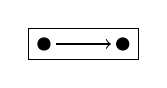
\begin{tikzpicture}
    \node[draw, rectangle, minimum width=1.4cm, minimum height=0.4cm] (boxT) {}; % Cuadro más grande para ajustarse a los puntos
    \node[fill=black, circle, inner sep=1.7pt] at (-0.5, 0) {}; % Primer punto a la izquierda
    \node[fill=black, circle, inner sep=1.7pt] at (0.5, 0) {}; % Segundo punto a la derecha
    \draw[->] (-0.35, 0) -- (0.35, 0); % Flecha con punta entre los dos puntos
\end{tikzpicture}}$ es una categoría con dos objetos y un morfismo entre ellos. 

Podemos usar esta filosofía para representar las estructuras iniciales de productos y equalizers en una categoría $\mathscr{C}$:

$$
    \textbf{P} = 
    \raisebox{0.1cm}{
    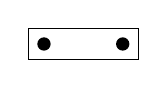
\begin{tikzpicture}[baseline=(current bounding box.center)]
        \node[draw, rectangle, minimum width=1.4cm, minimum height=0.4cm] (boxT) {};
        \node[fill=black, circle, inner sep=1.7pt] at (-0.5, 0) {};
        \node[fill=black, circle, inner sep=1.7pt] at (0.5, 0) {};
    \end{tikzpicture}}
    \hspace{0.5cm} \text{,} \hspace{0.5cm}
    \textbf{E} = 
    \raisebox{0.1cm}{
    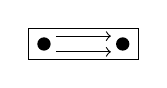
\begin{tikzpicture}[baseline=(current bounding box.center)]
        \node[draw, rectangle, minimum width=1.4cm, minimum height=0.4cm] (boxT) {};
        \node[fill=black, circle, inner sep=1.7pt] at (-0.5, 0) {};
        \node[fill=black, circle, inner sep=1.7pt] at (0.5, 0) {};
        \draw[->] (-0.35, 0.1) -- (0.35, 0.1);
        \draw[->] (-0.35, -0.1) -- (0.35, -0.1);
    \end{tikzpicture}}
$$

Un functor $\textbf{P} \longrightarrow \mathscr{C}$ consiste en los datos \eqref{data:iniciales-producto} y otro $\textbf{E} \longrightarrow \mathscr{C}$ consiste en los datos \eqref{data:iniciales-equalizer}.

\begin{definicion} [Diagrama]
    Sea $\mathscr{C}$ una categoría e \textbf{I} una categoría pequeña. Diremos que un functor $\textbf{I} \longrightarrow \mathscr{C}$ es un diagrama en $\mathscr{C}$ de forma \textbf{I}.
\end{definicion}

Luego \eqref{data:iniciales-producto} y \eqref{data:iniciales-equalizer} son diagramas de forma \textbf{P} y \textbf{E} respectivamente.

\begin{definicion}
    Sea $\mathscr{C}$ una categoría, \textbf{I} una categoría pequeña y $D: \textbf{I} \longrightarrow \mathscr{C}$ un diagrama en $\mathscr{C}$.

    \begin{enumerate}
        \item Un \textbf{cono} sobre $D$ es un objeto $C \in \mathscr{C}$ junto con una familia
        
        \begin{equation} \label{limit:cono}
            \left( C \overset{q_I}{\longrightarrow} D(I)\right)_{I \in \textbf{I}}
        \end{equation}

        de morfismos de forma que para todo morfismo $u: I \longrightarrow J$ en \textbf{I}, $q_J = D(u) \circ q_I$.

        \item Un \textbf{límite} de $D$ es un cono $\left(L, (p_I)_{I \in \textbf{I}}\right)$ con la propiedad de que para cualquier otro cono de la forma \eqref{limit:cono}, existe un único morfismo $c: C \longrightarrow L$ de forma que para todo objeto $I \in \textbf{I}$ se cumple $q_I = p_I \circ c$.

    \end{enumerate}
\end{definicion}

Esta definición generaliza y abstrae los conceptos de producto y equalizer, unificándolos dentro de un mismo marco teórico. 

Otro ejemplo familiar de límite en una categroía es el siguiente.

\begin{observacion}
    La categoría $(\mathbb{N}, \leq)$ tiene como objetos a los números naturales, y para cada par de objetos $n,m$ un morfismo $n \longrightarrow m$ si $n \leq m$. Por tanto, la categoría $(\mathbb{N}, \leq)^{op}$ tiene los mismos objetos y morfismos $n \longrightarrow m$ si $m \leq n$.
\end{observacion}

\begin{ejemplo}
    Sea $\textbf{I} = (\mathbb{N}, \leq)^{op}$, $\mathscr{C} = \textbf{Set}$ y un diagrama $D: \textbf{I} \longrightarrow \textbf{Set}$ que asocia a cada $n \in \textbf{I}$ un conjunto $X_n$, y a cada morfismo  $n \longrightarrow m$ (recordemos que entonces $m \leq n$) la función inclusión $X_n \subseteq X_m$. Resulta evidente que el conjunto $X_0$ asociado al objeto $0 \in \textbf{I}$ contiene al resto de conjuntos del diagrama. De hecho, se tiene la cadena de inclusiones

    \begin{equation}
        X_{n+1} \subseteq X_n \subseteq \dots \subseteq X_2 \subseteq X_1 \subseteq X_0 \text{.}
    \end{equation}

    El límite del diagrama $D$ será el conjunto intersección $\bigcap_{i \in \mathbb{N}} X_i $ de todos los conjuntos.

\end{ejemplo}

Como ha sido habitual en este capítulo, incluimos la definición del concepto dual de límite: el colímite.

\begin{definicion} 
    Sea $\mathscr{C}$ una categoría, \textbf{I} una categoría pequeña y $D: \textbf{I} \longrightarrow \mathscr{C}$ un diagrama en $\mathscr{C}$.
    \begin{enumerate}
        \item Un \textbf{cocono} sobre $D$ es un objeto $C \in \mathscr{C}$ junto con una familia
        
        \begin{equation} \label{colimit:cocono}
            \left( D(I) \overset{q_I}{\longrightarrow} C\right)_{I \in \textbf{I}}
        \end{equation}

        de morfismos de forma que para todo morfismo $u: I \longrightarrow J$ en \textbf{I}, $q_I = q_J \circ D(u)$.

        \item Un \textbf{colímite} de $D$ es un cocono $\left(L, (p_I)_{I \in \textbf{I}}\right)$ con la propiedad de que para cualquier otro cocono de la forma \eqref{colimit:cocono}, existe un único morfismo $c: L \longrightarrow C$ tal que para todo objeto $I \in \textbf{I}$ se cumple $q_I = c \circ p_I$.
    \end{enumerate}
\end{definicion}  

\section{Adjunciones}
Otro concepto categórico que jugará un papel fundamental en las etapas posteriores de este trabajo es el de functores adjuntos. Una adjunción describe una relación especial entre dos functores que permite establecer correspondencias naturales entre los morfismos de dos categorías diferentes. Este tipo de relación no solo facilita el paso de información de una categoría a otra, sino que también preserva estructuras algebraicas y topológicas de manera coherente.

Un caso particularmente importante que veremos más adelante es la adjunción entre el functor realización geométrica y el functor singular. Esta adjunción es clave para comprender cómo se trasladan conceptos algebraicos entre categorías, y cómo este paso de información puede ser aprovechado en el análisis topológico de datos.

\begin{definicion}
    Sean \begin{tikzcd}
        \mathscr{B} \arrow[shift left]{r}{F} & \mathscr{C} \arrow[shift left]{l}{G}
    \end{tikzcd} categorías y functores. Decimos que $F$ es adjunto por la izquierda a $G$ y $G$ es adjunto por la derecha a $F$, escribiendo $F \dashv G$, si para todo $B \in \mathscr{B}$ y $C \in \mathscr{C}$, existe un isomorfismo:
    
    \begin{equation}
        \mathscr{C}(F(B),C) \cong \mathscr{B}(B,G(C)),
    \end{equation}
    
    que es \textbf{natural} en $B$ y $C$, es decir, satisface:
    
    1. \textbf{Naturalidad en $B$}: Para todo morfismo $f: B' \to B$ en $\mathscr{B}$, el siguiente diagrama conmuta:
    \[
    \begin{tikzcd}[column sep=large]
        \mathscr{C}(F(B), C) \arrow{r}{\sim} \arrow{d}{F(f)^*} & \mathscr{B}(B, G(C)) \arrow{d}{f^*} \\
        \mathscr{C}(F(B'), C) \arrow{r}{\sim}                     & \mathscr{B}(B', G(C))
    \end{tikzcd}
    \]
    
    2. \textbf{Naturalidad en $C$}: Para todo morfismo $g: C \to C'$ en $\mathscr{C}$, el siguiente diagrama conmuta:
    \[
    \begin{tikzcd}[column sep=large]
        \mathscr{C}(F(B), C) \arrow{r}{\sim} \arrow{d}{g_*} & \mathscr{B}(B, G(C)) \arrow{d}{G(g)_*} \\
        \mathscr{C}(F(B), C') \arrow{r}{\sim}                  & \mathscr{B}(B, G(C'))
    \end{tikzcd}
    \]
    
    donde:
    \begin{itemize}
        \item $F(f)^*$ denota precomposición con $F(f)$,
        \item $f^*$ denota precomposición con $f$,
        \item $g_*$ denota poscomposición con $g$,
        \item $G(g)_*$ denota poscomposición con $G(g)$.
    \end{itemize}

\end{definicion}


\section{Categorías abelianas}

Introducimos ahora un tipo de categoría central para el desarrollo de nuestras ideas: las categorías abelianas. Estas estructuras serán fundamentales en nuestro enfoque categórico de la homología persistente, proporcionando un marco adecuado para el estudio de exactitud y homología en un contexto abstracto.


\begin{definicion} [Monomorfismo]
    Sea $\mathscr{C}$ una categoría y $f: A \longrightarrow B$ un morfismo en $\mathscr{C}$. Diremos que $f$ es un \textbf{monomorfismo} si dado un objeto $C$ y morfismos $g,h: C \longrightarrow A$ se cumple la siguiente propiedad:

    \begin{equation}
        (f \circ g = f \circ h) \Rightarrow (g = h)
    \end{equation}

    Usaremos el símobolo $f: A \rightarrowtail B$ para indicar que $f$ es un monomorfismo.
\end{definicion}

\begin{definicion} [Epimorfismo]
    Sea $\mathscr{C}$ una categoría y $f: A \longrightarrow B$ un morfismo en $\mathscr{C}$. Diremos que $f$ es un \textbf{epimorfismo} si, dado un objeto $C$ y morfismos $g,h: B \longrightarrow C$, se cumple la siguiente propiedad:

    \begin{equation}
        (g \circ f = h \circ f) \Rightarrow (g = h)
    \end{equation}

    Usaremos el símbolo $f: A \twoheadrightarrow B$ para indicar que $f$ es un epimorfismo.
\end{definicion}


\begin{proposicion}
    En una categoría $\mathscr{C}$, cuando dos morfismos \begin{tikzcd}
        f,g: A \arrow[r, shift left]{f} \arrow[r, shift right]{g} & B
    \end{tikzcd} tienen equalizer $(K,k)$, el morfismo $k: K \longrightarrow A$ es un monomorfismo.
\end{proposicion}
\begin{proof}
    Sean \begin{tikzcd}
        u,v: C \arrow[r, shift left]{f} \arrow[r, shift right]{g} & K
    \end{tikzcd} morfismos y supongamos que se cumple 
    \begin{equation} \label{hipo:mono}
        k \circ u = k \circ v\text{.}
    \end{equation}
    Queremos probar que entonces $u = v$. Como $(K,k)$ es equalizer de $f,g$ se cumple $f \circ k = g \circ k$, luego componiendo a la derecha con $u$ y $v$ se preserva la igualdad

    \begin{equation} \label{demo:monomorfismo}
        f \circ k \circ u = g \circ k \circ u \text{.}
    \end{equation}

    Tenemos que $(C, k \circ u) = (C, k \circ v)$, por \eqref{hipo:mono}, es una dupla que cumple \eqref{demo:monomorfismo} y como $(K,k)$ es el equalizer de $f,g$, por la propiedad universal de este límite existe un único morfismo $s: C \longrightarrow K$ cumpliendo

    \begin{equation} \label{propiedad:uni}
        k \circ s = k \circ u = k \circ v \text{.}
    \end{equation}

    Como $u$ y $k$ también cumplen \eqref{propiedad:uni}, la propiedad universal nos dice que necesariamente $s = u = v$, concluyendo la demostración.
\end{proof}

De forma análoga se demuestra la propiedad dual: En una categoría $\mathscr{C}$, cuando dos morfismos \begin{tikzcd}
    f,g: A \arrow[r, shift left]{f} \arrow[r, shift right]{g} & B
\end{tikzcd} tienen un coequalizer $(K,k)$, el morfismo $k: B \longrightarrow K$ es un epimorfismo.

\begin{definicion}
    Un \textbf{objeto cero} en una categoría $\mathscr{C}$ es un objeto $\boldsymbol{0}$ que es inicial y final al mismo tiempo. 
\end{definicion}

Notar que la definición de objeto cero es \textit{autodual}: se preserva en la categoría opuesta $\mathscr{C}^{op}$.

\begin{definicion}
    Sea una categoría $\mathscr{C}$ con un objeto $\boldsymbol{0}$. Un morfismo $f: A \longrightarrow B$ es un \textbf{morfismo cero} cuando factoriza a través del objeto $\boldsymbol{0}$. Es decir, el diagrama \ref{diag:zero-morphism} es conmutativo. 
\end{definicion}

\begin{figure}[h!]
    \centering
    \begin{tikzcd}
        & \boldsymbol{0} \arrow{rd} \\
        A \arrow{ru} \arrow{rr}[swap]{0_{A,B}} & & B
    \end{tikzcd}
    \caption{Diagrama conmutativo para morfismo cero}
    \label{diag:zero-morphism}
\end{figure}


\begin{proposicion} \label{unicidad-morfismo-cero}
    En una categoria $\mathscr{C}$ con un objeto cero $\boldsymbol{0}$, hay un único morfismo cero de cada objeto $A$ a cada objeto $B$.
\end{proposicion}
Sabemos que hay por lo menos un morfismo cero, digamos $0_{A,B}$, definido como la composición de los morfismos $A \longrightarrow \boldsymbol{0}$ y $\boldsymbol{0} \longrightarrow B$. Cualquier otro morfismo cero $f: A \longrightarrow B$ factoriza, por definición, a través del objeto cero. Es decir, se cumple la relación 

$$
    f = (\boldsymbol{0} \longrightarrow B) \circ (A \longrightarrow \boldsymbol{0}) \text{.}
$$

Para concluir $0_{A,B} = (A \longrightarrow \boldsymbol{0}) \circ (\boldsymbol{0} \longrightarrow B) = f$.

\begin{observacion}
    A ``el'' morfismo cero entre dos objetos $A$ y $B$ lo notaremos $0_{A,B}$.
\end{observacion}

\begin{proposicion} \label{composicion-es-cero}
    En una categoría $\mathscr{C}$ con un objeto cero $\boldsymbol{0}$, la composición de un morfismo cero con un morfismo arbitrario es de nuevo un morfismo cero.
\end{proposicion}
\begin{proof}
    Sea $f: A \longrightarrow B$ un morfismo cualquiera y $0_{B,C}: B \longrightarrow C$ el morfismo cero correspondiente. Por composición de morfismos y la definición de morfismo cero tenemos:

    \begin{equation}
        0_{B,C} \circ f = \left(0_{C} \circ 0_{B}\right) \circ f 
    \end{equation}

    Aplicando asociatividad en la composición:

    \begin{equation}
        0_{B,C} \circ f = \left(0_{C} \circ 0_{B}\right) \circ f =  0_{C} \circ \left(0_{B} \circ f\right)
    \end{equation}

    donde $\left(0_{B} \circ f\right) : A \longrightarrow \boldsymbol{0}$, pero por definición de $\boldsymbol{0}$, existe un único morfismo $0_{A}: A \longrightarrow \boldsymbol{0}$ luego $\left(0_{B} \circ f\right) = 0_A$. Obtenemos de esta forma la igualdad

    $$
    0_{B,C} \circ f =  0_{C} \circ \left(0_{B} \circ f\right) = 0_{C} \circ 0_{A}
    $$

     que demuestra que $0_{B,C} \circ f$ es un morfismo cero.
\end{proof}


\begin{definicion}
    En una categoría $\mathscr{C}$ con un objeto cero  $\boldsymbol{0}$, el núcleo de un morfismo $f: A \longrightarrow B$ es, cuando exista, el equalizer de $f$ y el morfismo cero $0_{A,B}: A \longrightarrow B$. Al objeto lo notaremos $Ker(f)$ y el morfismo asociado será $k: Ker(f) \longrightarrow A$. El cokernel se define de forma dual.
\end{definicion}

Indicamos ahora algunas observaciones triviales de esta definición.

\begin{proposicion} \label{mono}
    Sea $f: A \longrightarrow B$ un monomorfismo de una categoría $\mathscr{C}$ con un objeto cero $\boldsymbol{0}$. Si $f \circ g = 0_{C,B}$ para un morfismo $g: C \longrightarrow A$, entonces $g = 0_{C,A}$.
\end{proposicion}
\begin{proof}
    Por hipótesis asumimos que $f \circ g = 0_{C,B}$ y $f$ es monomorfismo. 
    
    Sea $f: A \longrightarrow B$ y $g: C \longrightarrow A$ un morfismo cualquiera. Por \ref{unicidad-morfismo-cero} existe $0_{C,A}: C \longrightarrow A$, y por \ref{composicion-es-cero} sabemos que $f \circ 0_{C,A} = 0_{C,B} = f \circ g$. Como $f$ es un monomorfismo, necesariamente $g = 0_{C,A}$. 
\end{proof}

\begin{proposicion} \label{monomorfismo-tiene-nucleo-0}
    En una categoría con un objeto cero $\boldsymbol{0}$, el núcleo de un monomorfismo $f: A \longrightarrow B$ es el morfismo $\boldsymbol{0} \longrightarrow A$.
\end{proposicion}
\begin{proof}
    Recordemos que el núcleo de $f: A \longrightarrow B$ es $(Ker(f),k)$ que cumple $f \circ k = 0_{A,B} \circ k$. Por \ref{composicion-es-cero} tenemos que $0_{A,B} \circ k = 0_{Ker(f),B} = f \circ k$ y por \ref{mono} aseguramos que $k = 0_{Ker(f),A}$. De esta forma, $k$ factoriza a través de $\boldsymbol{0}$ \begin{tikzcd}
        Ker(f) \arrow{r}{k} \arrow{d} & A \\
        \boldsymbol{0} \arrow{ur}
    \end{tikzcd}
    por la definición de morfismo cero, luego el objeto cero $\boldsymbol{0}$ cumple con la propiedad universal del equalizer y aseguramos que $Ker(f) = \boldsymbol{0}$.
\end{proof}

Vamos a ver algunos ejemplos para aclarar las nociones anteriormente presentadas.

\begin{ejemplo}
    En la categoría \textbf{Grp} de grupos y homomorfismos de grupos, el grupo trivial es un objeto cero y los morfismos cero son precisamente aquellos que llevan cualquier elemento en el elemento cero del grupo.

    Dado un homomorfismo de grupos $f: A \longrightarrow B$, su núcleo, según nuestra definición, es el equalizer de $f$ y el morfismo trivial. Esto es

    \begin{equation}
        Ker(f) = {a \in A | f(a) = 0} \text{.}
    \end{equation}
\end{ejemplo}

Una vez presentados los enunciados que tomaremos de base, procedemos a definir el concepto de categoría abeliana. 

\begin{definicion} [Categoría preaditiva]
     Una categoría preaditiva es una categoria $\mathscr{C}$ equipada con estructura de grupo en cada conjunto $\mathscr{C}(A,B)$ de forma que la composición de morfismos es bilineal: 

    \begin{equation}
        f \circ (g + h) = (f \circ g) + (f \circ h) \text{.}
    \end{equation}
\end{definicion}

Claramente, que cualquier categoría de modulos sobre un anillo es preaditiva.

Introducimos ahora una noción importante en categorías abelianas.

\begin{definicion}
    Sean $A$ y $B$ dos objetos en una categoría preaditiva $\mathscr{C}$. Un biproducto de $A$ y $B$ es una quíntupla $(P, p_A, p_B, s_A, s_B)$, donde:
    \begin{itemize}
        \item $P$ es un objeto de $\mathscr{C}$,
        \item $p_A: P \to A$ y $p_B: P \to B$ son morfismos llamados \textbf{proyecciones},
        \item $s_A: A \to P$ y $s_B: B \to P$ son morfismos llamados \textbf{secciones},
    \end{itemize}
    que satisfacen las siguientes identidades:  
    \begin{equation}
        p_A \circ s_A = \operatorname{id}_A, \quad 
        p_B \circ s_B = \operatorname{id}_B, \quad 
        p_A \circ s_B = 0, \quad 
        p_B \circ s_A = 0, \quad 
        s_A \circ p_A + s_B \circ p_B = \operatorname{id}_P.
    \end{equation}
    Cuando existe tal estructura, denotamos el biproducto como $A \oplus B$.
\end{definicion}


El biproducto en una categoría preaditiva abstrae la noción de suma directa en contextos algebraicos. La existencia de un biproducto para un par de objetos $A,B$ fuerza a que, si existe el producto de $A,B$, obligatoriamente es también coproducto y viceversa. 

En la categoría de módulos sobre un anillo $\mathbf{Mod}_R$, el biproducto $M \oplus N$ coincide con la suma directa usual de módulos, y en la categoría de grupos abelianos, representa la suma (o producto) directa de grupos. 

Notar que en la categoría \textbf{Grp}, el producto directo no es un coproducto, ya que para cumplir la propiedad universal necesitaría conmutatividad en los grupos.


\begin{definicion} [Categoría aditiva]
    Por categoría aditiva entendemos una categoría preadtivia con objeto cero y biproductos binarios para cada pareja de objetos.
\end{definicion}

Ya estamos en condiciones de definir el concepto central de esta sección.

\begin{definicion} [Categoría abeliana]
   Una categoría $\mathscr{C}$ se dice abeliana si se cumplen las siguientes condiciones:

    \begin{enumerate}
        \item $\mathscr{C}$ es una categoría aditiva;
        \item Cada morfismo en $\mathscr{C}$ tiene núcleo y conúcleo;
        \item Cada monomorfismo en $\mathscr{C}$ es un núcleo, y cada epimorfismo en $\mathscr{C}$ es un conúcleo.
    \end{enumerate}
\end{definicion}

Ahora que hemos establecido la noción de categoría abeliana, introducimos algunos conceptos adicionales sobre categorías que serán fundamentales para el desarrollo posterior relativo a álgebra homológica. 

\begin{proposicion} \label{proposicion-usual}
    Para un morfismo $f: A \longrightarrow B$ en una categoría abeliana $\mathscr{C}$, las siguientes condiciones equivalen:

    \begin{enumerate}
        \item $f$ es un monomorfismo;
        \item $Ker(f) = 0$
        \item $\forall C \in \mathscr{C} \quad \forall g: C \longrightarrow A \quad f \circ g = 0 \Rightarrow g = 0$
    \end{enumerate}
\end{proposicion}
\begin{proof}
    $(1) \Rightarrow (2)$ se probó en \ref{monomorfismo-tiene-nucleo-0} y $(1) \Rightarrow (3)$ se probó en \ref{mono}. 
    
    Vamos a probar $(2) \Rightarrow (1)$. Si $Ker(f) = 0$, sean dos morfismos $u,v$ tales que $f \circ u = f \circ v$ y su coequalizer $Coker(u,v) = q$ \footnote{La existencia del coequalizador de u y v no está garantizada en una categoría arbitraria. Sin embargo, en una categoría abeliana, que es completa y cocompleta, existen todos los límites y colímites pequeños. Para una demostración de este resultado, véase Handbook of Categorical Algebra II de Borceux, Capítulo 1, Sección 5, Proposición 1.5.3. Para una discusión general sobre categorías completas y cocompletas, consúltese Handbook of Categorical Algebra I, Capítulo 2, Sección 7.}. Como $q$ es un epimorfismo, $q = Coker(w)$ para algún $w$, por definición de categoría abeliana. Como $f \circ u = f \circ v$, por la propiedad universal del coequalizer $f$ debe factorizar a través de $q$ como $f = m \circ q$. Ya que $q = Coker(w)$ y por tanto $q \circ w = 0$, tenemos $f \circ w = m \circ q \ circ w = m \circ 0$. Esta relación nos dice que necesariamente $w$ de factorizar a través del núcleo de $f$: $w = k \circ n$. Al ser $Ker(f) = 0$ por hipótesis, necesariamente $w = 0$. Luego $q$ es el conúcleo de un morfismo cero, lo que nos indica que necesariamente debe ser la identidad sobre $B$, que a su vez es trivialmente un isomorfismo. Más concretamente, $q = id_B$ es un monomorfismo, y como $q \circ u = q \circ v$, entonces necesariamente $u = v$, probando así que $f$ es un monomorfismo (Ver \ref{diagrama-dificil}).

    Finalmente vamos a probar $(3) \Rightarrow (2)$. Recordemos que $Ker(f)$ es el equalizer del diagrama
    
    \begin{tikzcd}
        \boldsymbol{Ker(f)} \arrow{r}{k} & A \arrow[shift left]{r}{f} \arrow[shift right, swap]{r}{0_{A,B}} & B
    \end{tikzcd}
    cumpliendo $f \circ k = 0_{Ker(f),B}$. Por un lado tenemos un candidato en la composición 
    \begin{tikzcd}
        \boldsymbol{0} \arrow{r} & A \arrow{r}{f} & B
    \end{tikzcd}
    que es el morfismo cero asociado al objeto $B$, que sabemos que es único. Por otro lado si dado un objeto $C \in \mathscr{C}$ cualquiera y la composición
    \begin{tikzcd}
        C \arrow{r}{g} & A \arrow{r}{f} & B
    \end{tikzcd}
    es el morfismo $0_{C,B}$, por hipótesis en $(3)$ tenemos que $g = 0_{C,A}$. Nos queda entonces el siguiente diagrama
    \begin{tikzcd}
        C \arrow{r}{g} \arrow{d} & A \arrow{r}{f} & B \\
        \boldsymbol{0} \arrow{ur}
    \end{tikzcd}
    con $g$ factorizando a través del objeto cero, lo que prueba que dicho objeto cumple con la propiedad universal del equalizer y por tanto $Ker(f) = \boldsymbol{0}$.
\end{proof}

\begin{figure}[ht!]
    \centering
    \begin{tikzcd}
        Ker(f) \arrow{dr}{k} & \arrow[dotted]{l}[swap]{n} \arrow{d}{w} \bullet \\
        \bullet \arrow[shift right, swap]{r}{v} \arrow[shift left]{r}{u} & \bullet \arrow{r}{f} \arrow[twoheadrightarrow]{d}{q} & \bullet \\
        & \bullet \arrow[dotted]{ur}{m}
    \end{tikzcd}
    \caption{Diagrama que refleja la situación para \ref{proposicion-usual}}
    \label{diagrama-dificil}
\end{figure}

En el siguiente teorema se introduce un concepto conocido en categorías como \textbf{Ab} o $\mathbf{Mod}_R$: el objeto imagen de un morfismo. Aunque su definición puede parecer abstracta y distante de las nociones habituales, veremos que encapsula de manera general el concepto que buscamos.

\begin{teorema} \label{def:imagen}
    Todo morfismo $f$ en una categoría abeliana puede factorizarse de forma única (salvo isomorfismo) como $f = i \circ p$, donde $i$ es un monomorfismo y $p$ es un epimorfismo. De hecho, $i = Ker(Coker(f))$ y $p=Coker(Ker(f))$.
\end{teorema}
\begin{proof}
    La situación para esta demostración se encuentra reflejada en el diagrama \ref{diagrama-dificil-imagen}. Como $k$ es el morfismo asociado al núcleo de $f$, cumple $f \circ k = 0$. Por otro lado, $(Coker(k),p)$ es el conúcleo del morfismo $k: Ker(f) \longrightarrow A$ por lo que cumple $p \circ k = 0$. Por la propiedad universal del coequalizer se tiene que $f$ debe factorizar $f = i \circ p$ a través de $p$. Vamos a realizar el resto de la demostración por pasos.
    
    \begin{enumerate}
        \item \textbf{i es un monomorfismo}: Para ello, usando \ref{proposicion-usual}, es suficiente con tomar un morfismo $x$ cumpliendo $i \circ x = 0$ y demostrar que entonces $x = 0$. Como $i \circ x = 0$. Consideramos ahora $(Coker(x),q)$ el conúcleo del morfismo $x$ (recordemos que siempre existe debido a que nuestro ambiente es una categoría abeliana que en particular es cocompleta) de forma que al cumplirse $i \circ x = 0$, necesariamente $i$ debe factorizar $i = r \circ q$ a través de $q$ por la propiedad universal del coequalizer. Ahora tenemos que $p$ y $q$ son dos epimorfismos, por lo que la composición $q \circ p$ es también un epimorfismo. De nuevo al estar en una categoría abeliana, si $q \circ p$ es un epimorfismo, necesariamente existe $h$ tal que $q \circ p = Coker(h)$, donde $h$ tiene como codominio el objeto $A$. La relación
        
        \begin{equation}
            f \circ h = i \circ p \circ h = r \circ q \circ p \circ h = r \circ 0 = 0
        \end{equation}

        y la propiedad universal del equalizer inducen que $h$ debe factorizar $h = k \circ l$  a través de $k$. Finalmente $p \circ h = p \circ k \circ l = 0 \circ l = 0$, pero como $q \circ p = Coker(h)$, $p$ debe factorizar $p = s \circ (q \circ p)$. Como $p$ es un epimorfismo, por definición, si se cumple $p = (s \circ q) \circ p$, entonces $s \circ q = 1$. Luego $q$ es en particular un monomorfismo de donde $q \circ x = 0$ implica que $x = 0$, probando así que $i$ es un monomorfismo.
        
        \item \textbf{La factorización de $f$ es única}: Esta parte se prueba usando que los epimorfismos regulares son fuertes \footnote{Consúltese Handbook of Categorical Algebra I, Capítulo 4, Sección 4, Proposición 4.4.5}.
        
        Por un argumento de dualidad, $f$ factoriza como $f = i' \circ p'$ con $i' = Ker(Coker(f))$ y $p'$ un epimorfismo. Por unicidad, necesariamente las factorizaciones $f = i \circ p$ y $f = i' \circ p'$ son isomorfas.
    \end{enumerate}
\end{proof}

\begin{figure}[ht!]
    \centering
    \begin{tikzcd}
        & \arrow{dl}[swap]{l} \arrow{d}{h} \bullet \\
        Ker(f) \arrow{r}{k} & A \arrow{r}{f} \arrow{d}{p} & B \\
        \bullet \arrow{r}{x} & Coker(k) \arrow{ur}{i} \arrow[shift right, swap]{r}{q}& Coker(x) \arrow{u}{r} \arrow[shift right, swap]{l}{s}
    \end{tikzcd}
    \caption{Diagrama que refleja la situación para \ref{def:imagen}}
    \label{diagrama-dificil-imagen}
\end{figure}


\begin{observacion}
    La factorización de $f$ referida en \ref{def:imagen} se conoce como ``factorización imagen'' de $f$. Los morfismos $i$ y $p$ de la composición tienen por dominio y codominio respectivamente el objeto $Im(f)$. Por tanto $f(A)$ ``es'' el cociente de $A$ por el núcleo de f, i.e. el conúcleo del núcleo de $f$. 
\end{observacion}

\begin{observacion}
    Intuitivamente, tiene sentido definir la imagen de un morfismo como el conúcleo de su núcleo. Recordemos que el núcleo de un morfismo mide la parte del dominio que es enviada al morfismo cero, es decir, la información que se "pierde". Por otro lado, el conúcleo nos indica cuánto le falta a un morfismo para ser un epimorfismo. Así, el conúcleo del núcleo de un morfismo proporciona una medida de la parte del dominio que sobrevive tras eliminar la información perdida, capturando de manera abstracta la noción de imagen en términos categóricos.
\end{observacion}


\begin{ejemplo}
    En el caso de la categoría \textbf{Ab} de grupos abelianos y el homomorfismo de grupos $f: A \longrightarrow B$ tenemos la factorización $Im(f) = f(A)$ donde $p: A \longrightarrow f(A)$ es sobreyectivo y $i: f(A) \hookrightarrow B$ es inyectivo.
\end{ejemplo}

Vamos ahora a introducir unos objetos que serán centrales en este trabajo por su importancia en el álgebra homológica: las sucesiones exactas.

\begin{definicion} \label{secuencia-exacta}
    En $\mathscr{C}$ una categoría abeliana, un par de morfismos composables 

    \begin{equation}
        \begin{tikzcd}
            A \arrow{r}{f} & B \arrow{r}{g} & C
        \end{tikzcd}
    \end{equation}

    forman una \textbf{secuencia exacta}  si la imagen de $f$ coincide con el núcleo de $g$. 

    \begin{equation}
        \begin{tikzcd}
            A \arrow{r}{f} \arrow{d}{p} & B \arrow{r}{g} & C \\
            Im(f) \arrow{ur}{i} & Ker(f) \arrow{u}{k}
        \end{tikzcd}
    \end{equation}
\end{definicion}

\begin{definicion}
    Por \textbf{secuencia exacta corta} en una categoría abeliana $\mathscr{C}$ entendemos una secuencia exacta de la forma 

    \begin{equation}
        \begin{tikzcd}
            \boldsymbol{0} \arrow{r} & A \arrow{r}{f} & B \arrow{r}{g} & C \arrow{r} & \boldsymbol{0}
        \end{tikzcd}
    \end{equation}
\end{definicion}

\begin{definicion}
    Una secuencia de morfismos

    \begin{equation}
        \begin{tikzcd}
            \dots \arrow{r} & A_n \arrow{r}{f_n} & A_{n+1} \arrow{r}{f_{n+1}} & A_{n+2} \arrow{r} & \dots
        \end{tikzcd}
    \end{equation}

    es una \textbf{secuencia exacta larga} si cada par de morfismos consecutivos forma una secuencia exacta en el sentido de \ref{secuencia-exacta}.
\end{definicion}

\begin{lema}[Lema de la Serpiente]
    Sea la siguiente fila conmutativa de morfismos en una categoría abeliana $\mathscr{C}$, donde las filas son exactas:

    \begin{equation}
        \begin{tikzcd}
            & A \arrow{r}{f} \arrow{d}{a} & B \arrow{r}{g} \arrow{d}{b} & C \arrow{r}{} \arrow{d}{c} & \boldsymbol{0} \\
            \boldsymbol{0} \arrow{r} & A' \arrow{r}{f'} & B' \arrow{r}{g'} & C' &\\
        \end{tikzcd}
    \end{equation}
    
    Entonces existe una aplicación canónica, llamada \textbf{morfismo de conexión}, que asocia a cada secuencia exacta corta de arriba una secuencia exacta larga:

    \begin{equation}
        \begin{tikzcd}
            \ker a' \arrow[r]{r}{} & \ker a \arrow[r]{r}{} & \ker a'' \arrow[r]{r}{\delta} & \operatorname{coker} a' \arrow[r]{r}{} & \operatorname{coker} a \arrow[r]{r}{} & \operatorname{coker} a''.
        \end{tikzcd}
    \end{equation}
    
\end{lema}





\endinput
